%\title{beavtex}
\documentclass[double,12pt]{beavtex}
\usepackage{graphicx}
\usepackage{rotating} %Package added to allow the rotation of figures and chart on a page, {sidewaysfigure} command
\usepackage{tablefootnote} %Packaged added to allow footnotes in the tabular environment, use \tablefootnote command
\usepackage[round]{natbib}
\usepackage{booktabs}
\bibliographystyle{plainnat}
\title{An Analysis of Something}
\author{Joseph A. Student}
\degree{Master of Science}
\doctype{Thesis}
\department{Nuclear Engineering and Radiation Health Physics}
\depttype{School}
\depthead{Director}
\major{Radiation Health Physics}
\advisor{Jane R. Professor}
\advisor{Jane D. Professor}
\submitdate{January 1, 2013}
\commencementyear{2013}


\abstract{This is the place for the abstract text.}


\acknowledgements{I would like to acknowledge...Lorem ipsum dolor sit amet, consectetur adipiscing elit. Maecenas vel eros sed mauris porttitor semper nec a orci. Nullam vestibulum mi nec condimentum posuere. Pellentesque eget diam id sapien aliquet ullamcorper. Pellentesque blandit nec lectus ut mollis. Praesent in facilisis justo. Vestibulum ante ipsum primis in faucibus orci luctus et ultrices posuere cubilia Curae; Sed eget congue leo, sed consequat libero. In rutrum malesuada nisi. Vestibulum ante ipsum primis in faucibus orci luctus et ultrices posuere cubilia Curae; Morbi sollicitudin tortor ut sem facilisis mollis.}


\begin{document}
\maketitle
\mainmatter

%-------------------------INTRODUCTION-----------------------------

\chapter{Introduction}

\section{Objective}


The purpose of this study is to... Lorem~\citep{bockheimNutrientDynamicsDecomposing2011}, my butt is made of sand ~\citep{munsonNuCMCodeVersion1992} ipsum dolor sit amet, consectetur adipiscing elit. Sed venenatis nunc sapien. Praesent imperdiet nulla eu rutrum venenatis. Fusce rhoncus urna a nunc semper, non venenatis lorem tempor. Cras sollicitudin eget velit eu venenatis. Mauris imperdiet pretium massa sed dapibus. Nunc ipsum ipsum, porttitor ut urna ut, pretium feugiat leo. Nunc magna enim, facilisis a porttitor eget, elementum ac turpis. Quisque et gravida justo. Etiam vulputate quam at commodo suscipit. Vivamus ut adipiscing tortor. Phasellus quis dolor et mi hendrerit sollicitudin. 

Cras dapibus congue mauris, et imperdiet magna pellentesque non. Sed venenatis adipiscing quam ut placerat. Praesent imperdiet dignissim cursus. Phasellus mattis nibh vitae semper pellentesque. Lorem ipsum dolor sit amet, consectetur adipiscing elit. Sed dignissim tellus id adipiscing tempus. Aenean posuere malesuada rhoncus. Ut quis elit eros.


\section{Background}

Lorem ipsum dolor sit amet, consectetur adipiscing elit. Sed venenatis nunc sapien. Praesent imperdiet nulla eu rutrum venenatis. Fusce rhoncus urna a nunc semper, non venenatis lorem tempor. Cras sollicitudin eget velit eu venenatis. Mauris imperdiet pretium massa sed dapibus. Nunc ipsum ipsum, porttitor ut urna ut, pretium feugiat leo. Nunc magna enim, facilisis a porttitor eget, elementum ac turpis. Quisque et gravida justo. Etiam vulputate quam at commodo suscipit. Vivamus ut adipiscing tortor. Phasellus quis dolor et mi hendrerit sollicitudin. 

Cras dapibus congue mauris, et imperdiet magna pellentesque non. Sed venenatis adipiscing quam ut placerat. Praesent imperdiet dignissim cursus. Phasellus mattis nibh vitae semper pellentesque. Lorem ipsum dolor sit amet, consectetur adipiscing elit. Sed dignissim tellus id adipiscing tempus. Aenean posuere malesuada rhoncus. Ut quis elit eros.



%------------------------LIT REVIEW--------------------------------

\chapter{Literature Review}

\section{First Section of Lit Review}

Frogs are weird...

\begin{figure}[ht!]
\begin{center}
	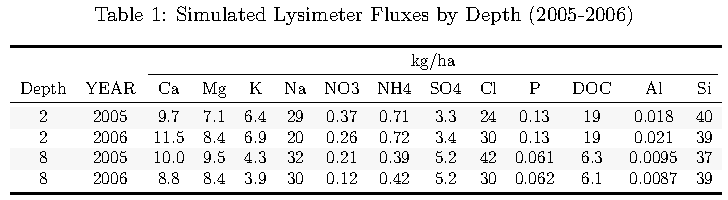
\includegraphics[width=20cm]{Images/LN_SED/Base/test.pdf}
	\caption{Frog pic...}
	\label{fig:frog}
	\end{center}
\end{figure}


Here is a reference to the from pic: Figure~\ref{fig:frog}.

\section{Just another section of this chapter.}

Lorem ipsum dolor sit amet, consectetur adipiscing elit. Sed venenatis nunc sapien. Praesent imperdiet nulla eu rutrum venenatis. Fusce rhoncus urna a nunc semper, non venenatis lorem tempor. Cras sollicitudin eget velit eu venenatis. Mauris imperdiet pretium massa sed dapibus. Nunc ipsum ipsum, porttitor ut urna ut, pretium feugiat leo. Nunc magna enim, facilisis a porttitor eget, elementum ac turpis. Quisque et gravida justo. Etiam vulputate quam at commodo suscipit. Vivamus ut adipiscing tortor. Phasellus quis dolor et mi hendrerit sollicitudin. 

Cras dapibus congue mauris, et imperdiet magna pellentesque non. Sed venenatis adipiscing quam ut placerat. Praesent imperdiet dignissim cursus. Phasellus mattis nibh vitae semper pellentesque. Lorem ipsum dolor sit amet, consectetur adipiscing elit. Sed dignissim tellus id adipiscing tempus. Aenean posuere malesuada rhoncus. Ut quis elit eros.



%-------------------MATERIALS & METHODS--------------------------

\chapter{Materials and Methods}

\section{Primary Methods}

Lorem ipsum dolor sit amet, consectetur adipiscing elit. Sed venenatis nunc sapien. Praesent imperdiet nulla eu rutrum venenatis. Fusce rhoncus urna a nunc semper, non venenatis lorem tempor. Cras sollicitudin eget velit eu venenatis. Mauris imperdiet pretium massa sed dapibus. Nunc ipsum ipsum, porttitor ut urna ut, pretium feugiat leo. Nunc magna enim, facilisis a porttitor eget, elementum ac turpis. Quisque et gravida justo. Etiam vulputate quam at commodo suscipit. Vivamus ut adipiscing tortor. Phasellus quis dolor et mi hendrerit sollicitudin. 

Cras dapibus congue mauris, et imperdiet magna pellentesque non. Sed venenatis adipiscing quam ut placerat. Praesent imperdiet dignissim cursus. Phasellus mattis nibh vitae semper pellentesque. Lorem ipsum dolor sit amet, consectetur adipiscing elit. Sed dignissim tellus id adipiscing tempus. Aenean posuere malesuada rhoncus. Ut quis elit eros.


\begin{table}[ht]
\caption{Types of stuff you put in a table} % title of Table
\centering  % used for centering table
\begin{tabular}{c c} % centered columns (2 columns)
\hline\hline                        %inserts double horizontal lines
Header 1 & Header 2 \\ [0.5ex] % inserts table heading
\hline                  % inserts single horizontal line
Item 1 & something  \\ % inserting body of the table
Item 2 & something else  \\
Item 3 & more things  \\
Item 4 & and more \\
Item 5 & last thing \\ [1ex]      % [1ex] adds vertical space
\hline %inserts single line
\end{tabular}
\label{table:misc} % is used to refer this table in the text
\end{table}


\begin{table}[ht]
\centering
\caption{Thicker horizontal lines above and below the table.}
\begin{tabular}[t]{lcc}
\toprule
&Treatment A&Treatment B\\
\midrule
John Smith&1&2\\
Jane Doe&--&3\\
Mary Johnson&4&5\\
\bottomrule
\end{tabular}
\end{table}%


\section{More Methods}

Lorem ipsum dolor sit amet, consectetur adipiscing elit. Sed venenatis nunc sapien. Praesent imperdiet nulla eu rutrum venenatis. Fusce rhoncus urna a nunc semper, non venenatis lorem tempor. Cras sollicitudin eget velit eu venenatis. Mauris imperdiet pretium massa sed dapibus. Nunc ipsum ipsum, porttitor ut urna ut, pretium feugiat leo. Nunc magna enim, facilisis a porttitor eget, elementum ac turpis. Quisque et gravida justo. Etiam vulputate quam at commodo suscipit. Vivamus ut adipiscing tortor. Phasellus quis dolor et mi hendrerit sollicitudin. 

Cras dapibus congue mauris, et imperdiet magna pellentesque non. Sed venenatis adipiscing quam ut placerat. Praesent imperdiet dignissim cursus. Phasellus mattis nibh vitae semper pellentesque. Lorem ipsum dolor sit amet, consectetur adipiscing elit. Sed dignissim tellus id adipiscing tempus. Aenean posuere malesuada rhoncus. Ut quis elit eros.


%------------------------RESULTS--------------------------------

\chapter{Results}

Lorem ipsum dolor sit amet, consectetur adipiscing elit. Fusce posuere sed magna sit amet hendrerit. Integer gravida mattis posuere. Pellentesque at libero consectetur, pulvinar augue ac, pharetra augue. Cras fermentum augue id odio rutrum, eget eleifend lectus adipiscing. Duis libero massa, rutrum eget purus eu, tempus dapibus dolor. Class aptent taciti sociosqu ad litora torquent per conubia nostra, per inceptos himenaeos. Sed aliquet fringilla odio at euismod. Etiam viverra convallis tortor, hendrerit varius nulla pharetra ac. 

Donec vitae mollis sem, non viverra arcu. Integer vel risus justo. Proin consectetur justo nisl, ut auctor mauris rhoncus id. Vestibulum eget egestas risus. Nullam eget nunc non tortor pretium rhoncus dapibus eu orci. In hendrerit velit vel turpis vulputate porttitor. Praesent commodo, neque at porta posuere, ligula ipsum euismod dolor, ac pharetra erat purus non nunc. Praesent placerat placerat fermentum. Class aptent taciti sociosqu ad litora torquent per conubia nostra, per inceptos himenaeos. Praesent volutpat, purus id molestie egestas, mauris neque accumsan tellus, vitae fermentum lorem neque a lectus. Morbi tincidunt metus dui, vitae adipiscing mauris porttitor vitae. Donec a dolor convallis, tincidunt sapien vel, malesuada lorem. Fusce a magna sit amet leo accumsan dapibus at nec tellus. Nam id erat at ligula adipiscing porttitor in semper augue. Etiam imperdiet lobortis dui, a ornare lorem vulputate vitae. 

Etiam non libero in leo egestas porta et eu nunc. Duis molestie suscipit semper. Vestibulum nec sodales odio, vestibulum sagittis lacus. Phasellus volutpat, velit in pretium malesuada, nibh magna consequat neque, in interdum magna mi at erat. In hac habitasse platea dictumst. Praesent consectetur ut lorem sagittis tempus. Ut venenatis eu mi eget sollicitudin. Praesent posuere non lorem nec lacinia. Nunc at vulputate dolor. Aliquam et dolor sit amet quam viverra condimentum vitae eu dui. Quisque pellentesque purus in tortor vehicula sollicitudin. Curabitur sit amet vehicula diam. Vivamus mauris nulla, dictum ac ipsum eget, molestie scelerisque diam. Curabitur sit amet dolor nibh. Cum sociis natoque penatibus et magnis dis parturient montes, nascetur ridiculus mus. Sed semper sed diam quis feugiat. 


\begin{equation}
MDC=\frac{3.29*\sqrt{(Bkgcpm*C_{t}*(1+\frac{C_{t}}{BkgC_{t}}))}+3.0}{2.22*E*C_{t}*V*decay*A*R*DF*I}
\label{eq:mdc}
\end{equation}
Where:

\begin{itemize}
\item $C_{t} =$ Sample count time
\item $BkgC_{t} =$ Background count time
\item $Bkgcpm =$ Background counts per minute (cpm)
\item $E =$ Counting efficiency
\item $V =$ Sample volume or weight
\item $decay =$ isotopic decay (if applicable)
\item $A =$ Isotopic abundance (if applicable)
\item $R =$ Recovery (if applicable)
\item $DF =$ Dilution factor for liquid scintillation (if applicable)
\item $I =$ Additional decay or ingrowth factors (if applicable)
\end{itemize}

Lorem ipsum dolor sit amet, consectetur adipiscing elit. Sed venenatis nunc sapien. Praesent imperdiet nulla eu rutrum venenatis. Fusce rhoncus urna a nunc semper, non venenatis lorem tempor. Cras sollicitudin eget velit eu venenatis. Mauris imperdiet pretium massa sed dapibus. Nunc ipsum ipsum, porttitor ut urna ut, pretium feugiat leo. Nunc magna enim, facilisis a porttitor eget, elementum ac turpis. Quisque et gravida justo. Etiam vulputate quam at commodo suscipit. Vivamus ut adipiscing tortor. Phasellus quis dolor et mi hendrerit sollicitudin. 

Cras dapibus congue mauris, et imperdiet magna pellentesque non. Sed venenatis adipiscing quam ut placerat. Praesent imperdiet dignissim cursus. Phasellus mattis nibh vitae semper pellentesque. Lorem ipsum dolor sit amet, consectetur adipiscing elit. Sed dignissim tellus id adipiscing tempus. Aenean posuere malesuada rhoncus. Ut quis elit eros.


\pagebreak[4]

\begin{figure}
\begin{center}
	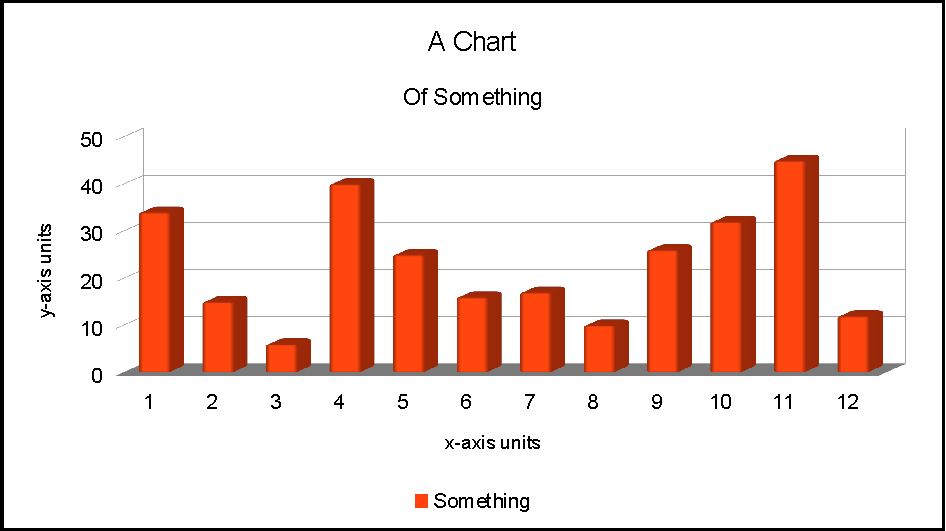
\includegraphics[width=14cm]{chart.pdf}
	\caption{A Chart.}
	\label{fig:chart}
	\end{center}
\end{figure}

\pagebreak[4]

\begin{sidewaysfigure}[htbp]
\begin{center}
	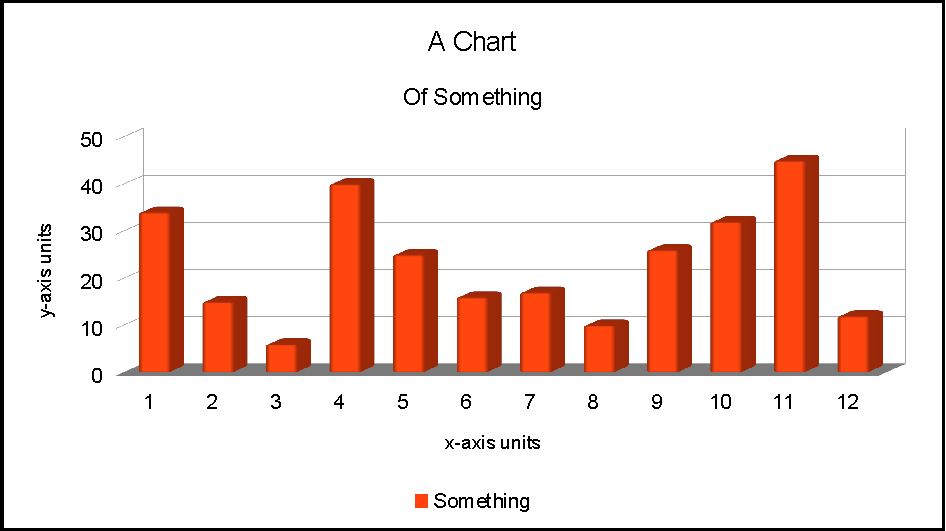
\includegraphics[width=18cm]{chart.pdf}
	\caption{Same chart, but using sidewaysfigure.}
	\label{fig:rain}
	\end{center}
\end{sidewaysfigure}


%-----------------------DISCUSSION--------------------------------

\chapter{Discussion}

\section{First Subsection}

Lorem ipsum dolor sit amet, consectetur adipiscing elit. Fusce posuere sed magna sit amet hendrerit. Integer gravida mattis posuere. Pellentesque at libero consectetur, pulvinar augue ac, pharetra augue. Cras fermentum augue id odio rutrum, eget eleifend lectus adipiscing. Duis libero massa, rutrum eget purus eu, tempus dapibus dolor. Class aptent taciti sociosqu ad litora torquent per conubia nostra, per inceptos himenaeos. Sed aliquet fringilla odio at euismod. Etiam viverra convallis tortor, hendrerit varius nulla pharetra ac. 

Donec vitae mollis sem, non viverra arcu. Integer vel risus justo. Proin consectetur justo nisl, ut auctor mauris rhoncus id. Vestibulum eget egestas risus. Nullam eget nunc non tortor pretium rhoncus dapibus eu orci. In hendrerit velit vel turpis vulputate porttitor. Praesent commodo, neque at porta posuere, ligula ipsum euismod dolor, ac pharetra erat purus non nunc. Praesent placerat placerat fermentum. Class aptent taciti sociosqu ad litora torquent per conubia nostra, per inceptos himenaeos. Praesent volutpat, purus id molestie egestas, mauris neque accumsan tellus, vitae fermentum lorem neque a lectus. Morbi tincidunt metus dui, vitae adipiscing mauris porttitor vitae. Donec a dolor convallis, tincidunt sapien vel, malesuada lorem. Fusce a magna sit amet leo accumsan dapibus at nec tellus. Nam id erat at ligula adipiscing porttitor in semper augue. Etiam imperdiet lobortis dui, a ornare lorem vulputate vitae. 

Etiam non libero in leo egestas porta et eu nunc. Duis molestie suscipit semper. Vestibulum nec sodales odio, vestibulum sagittis lacus. Phasellus volutpat, velit in pretium malesuada, nibh magna consequat neque, in interdum magna mi at erat. In hac habitasse platea dictumst. Praesent consectetur ut lorem sagittis tempus. Ut venenatis eu mi eget sollicitudin. Praesent posuere non lorem nec lacinia. Nunc at vulputate dolor. Aliquam et dolor sit amet quam viverra condimentum vitae eu dui. Quisque pellentesque purus in tortor vehicula sollicitudin. Curabitur sit amet vehicula diam. Vivamus mauris nulla, dictum ac ipsum eget, molestie scelerisque diam. Curabitur sit amet dolor nibh. Cum sociis natoque penatibus et magnis dis parturient montes, nascetur ridiculus mus. Sed semper sed diam quis feugiat. 

\begin{equation}
A(t)=A_{o}e^{(-\lambda t)}
\label{eq:initialeq}
\end{equation}

Then Equation~\ref{eq:initialeq} is integrated to become:

\begin{equation}
\tilde{C}=\int_0^{t}A(t)dt = \frac{A_{o}}{\lambda} (1-e^{(-\lambda t)})
\label{eq:finaleq}
\end{equation}

Where:

\begin{itemize}
\item $A(t) =$ original exponential function
\item $A_{o} =$ the peak activity at day 0 (Bq per mass or volume)
\item $\tilde{C} =$ Integrated Activity Concentration (Bq-days per mass or volume)
\item $t =$ 28 days
\item $\lambda =$ removal constant (day$^{-1}$)
\end{itemize}



\section{Another Subsection}

Lorem ipsum dolor sit amet, consectetur adipiscing elit. Fusce posuere sed magna sit amet hendrerit. Integer gravida mattis posuere. Pellentesque at libero consectetur, pulvinar augue ac, pharetra augue. Cras fermentum augue id odio rutrum, eget eleifend lectus adipiscing. Duis libero massa, rutrum eget purus eu, tempus dapibus dolor. Class aptent taciti sociosqu ad litora torquent per conubia nostra, per inceptos himenaeos. Sed aliquet fringilla odio at euismod. Etiam viverra convallis tortor, hendrerit varius nulla pharetra ac. 

Donec vitae mollis sem, non viverra arcu. Integer vel risus justo. Proin consectetur justo nisl, ut auctor mauris rhoncus id. Vestibulum eget egestas risus. Nullam eget nunc non tortor pretium rhoncus dapibus eu orci. In hendrerit velit vel turpis vulputate porttitor. Praesent commodo, neque at porta posuere, ligula ipsum euismod dolor, ac pharetra erat purus non nunc. Praesent placerat placerat fermentum. Class aptent taciti sociosqu ad litora torquent per conubia nostra, per inceptos himenaeos. Praesent volutpat, purus id molestie egestas, mauris neque accumsan tellus, vitae fermentum lorem neque a lectus. Morbi tincidunt metus dui, vitae adipiscing mauris porttitor vitae. Donec a dolor convallis, tincidunt sapien vel, malesuada lorem. Fusce a magna sit amet leo accumsan dapibus at nec tellus. Nam id erat at ligula adipiscing porttitor in semper augue. Etiam imperdiet lobortis dui, a ornare lorem vulputate vitae. 

Finally, a table with a footnote...

\begin{table}[htbp!]
\caption{Some table values}
\centering
\begin{tabular}{cccccc}
\hline\hline
 & & & & & Total \\
Sample & $A_{o}$\tablefootnote{some kind of footnote from a table, which doesn't work without the tablefootnote package} & $\lambda$ & $\tilde{C}$ & Something & (units) \\
\hline   \\
Item 1 & 1 & .55 & 3 & 125 & 70  \\
Item 2 & 1 & .55 & 3 & 125 & 70  \\
Item 3 & 1 & .55 & 3 & 125 & 70  \\
Item 4 & 1 & .55 & 3 & 125 & 70  \\ [1ex]
\hline
\textbf{Total} &  &  &  &  & \textbf{280} \\ [1ex]
\hline
\end{tabular}
\label{table:intake2}
\end{table}


Etiam non libero in leo egestas porta et eu nunc. Duis molestie suscipit semper. Vestibulum nec sodales odio, vestibulum sagittis lacus. Phasellus volutpat, velit in pretium malesuada, nibh magna consequat neque, in interdum magna mi at erat. In hac habitasse platea dictumst. Praesent consectetur ut lorem sagittis tempus. Ut venenatis eu mi eget sollicitudin. Praesent posuere non lorem nec lacinia. Nunc at vulputate dolor. Aliquam et dolor sit amet quam viverra condimentum vitae eu dui. Quisque pellentesque purus in tortor vehicula sollicitudin. Curabitur sit amet vehicula diam. Vivamus mauris nulla, dictum ac ipsum eget, molestie scelerisque diam. Curabitur sit amet dolor nibh. Cum sociis natoque penatibus et magnis dis parturient montes, nascetur ridiculus mus. Sed semper sed diam quis feugiat.




\chapter{Conclusion}

Lorem ipsum dolor sit amet, consectetur adipiscing elit. Fusce posuere sed magna sit amet hendrerit. Integer gravida mattis posuere. Pellentesque at libero consectetur, pulvinar augue ac, pharetra augue. Cras fermentum augue id odio rutrum, eget eleifend lectus adipiscing. Duis libero massa, rutrum eget purus eu, tempus dapibus dolor. Class aptent taciti sociosqu ad litora torquent per conubia nostra, per inceptos himenaeos. Sed aliquet fringilla odio at euismod. Etiam viverra convallis tortor, hendrerit varius nulla pharetra ac. 

Donec vitae mollis sem, non viverra arcu. Integer vel risus justo. Proin consectetur justo nisl, ut auctor mauris rhoncus id. Vestibulum eget egestas risus. Nullam eget nunc non tortor pretium rhoncus dapibus eu orci. In hendrerit velit vel turpis vulputate porttitor. Praesent commodo, neque at porta posuere, ligula ipsum euismod dolor, ac pharetra erat purus non nunc. Praesent placerat placerat fermentum. Class aptent taciti sociosqu ad litora torquent per conubia nostra, per inceptos himenaeos. Praesent volutpat, purus id molestie egestas, mauris neque accumsan tellus, vitae fermentum lorem neque a lectus. Morbi tincidunt metus dui, vitae adipiscing mauris porttitor vitae. Donec a dolor convallis, tincidunt sapien vel, malesuada lorem. Fusce a magna sit amet leo accumsan dapibus at nec tellus. Nam id erat at ligula adipiscing porttitor in semper augue. Etiam imperdiet lobortis dui, a ornare lorem vulputate vitae. 

Etiam non libero in leo egestas porta et eu nunc. Duis molestie suscipit semper. Vestibulum nec sodales odio, vestibulum sagittis lacus. Phasellus volutpat, velit in pretium malesuada, nibh magna consequat neque, in interdum magna mi at erat. In hac habitasse platea dictumst. Praesent consectetur ut lorem sagittis tempus. Ut venenatis eu mi eget sollicitudin. Praesent posuere non lorem nec lacinia. Nunc at vulputate dolor. Aliquam et dolor sit amet quam viverra condimentum vitae eu dui. Quisque pellentesque purus in tortor vehicula sollicitudin. Curabitur sit amet vehicula diam. Vivamus mauris nulla, dictum ac ipsum eget, molestie scelerisque diam. Curabitur sit amet dolor nibh. Cum sociis natoque penatibus et magnis dis parturient montes, nascetur ridiculus mus. Sed semper sed diam quis feugiat. 

\pagebreak

\bibliography{thesis}

\pagebreak

\appendix

\begin{table}[ht]
\centering
\caption{Sources of Parameterization}
\begin{tabular}[t]{cc}
\toprule
Parameter&Source\\
\midrule
Example Parameter& \cite{bockheimNutrientDynamicsDecomposing2011}\\
Example 2&3\\
4&5\\
\bottomrule
\end{tabular}
\end{table}%

\chapter{Things}





\chapter{More Things}





\end{document}